\documentclass[a4paper]{report}

\usepackage[swedish]{babel}
\usepackage{capt-of}
\usepackage{algorithm}
\usepackage{algpseudocode}
\usepackage{todonotes}
\usepackage[utf8]{inputenc}
\usepackage{graphicx}
\usepackage{titlesec}
\usepackage{xcolor}
\usepackage[parfill]{parskip}
\usepackage{hyperref}
\usepackage{amsmath}
\usepackage{amsthm}
\usepackage{cite}


\titleformat{\chapter}{\normalfont\LARGE\bfseries}{\thechapter.}{1em}{}
\newtheorem{theorem}{Sats}
\newtheorem{corollary}{Följdsats}

\title{Algoritmer för graffärgning}
\author{Johan Sannemo}
\date{}

\begin{document}
\begin{titlepage}
\begin{center}
\vspace*{1cm}
\Huge
\textbf{Hur man färgar grafer}
\vspace{0.5cm}
\large

En studie av algoritmer för att beräkna det kromatiska talet

\vspace{1.5cm}

\textbf{Johan Sannemo}


\end{center}
\vfill
\normalsize
Gymnasiearbete inom naturvetenskapsprogrammet - matematisk specialisering\\
Danderyds Gymnasium
\vspace{0.8cm}

\normalsize
Handledare: Ulf Backlund\\
Bihandledare: Per Austrin\\

\end{titlepage}

\clearpage
\section*{Abstract}
\textbf{Key words:} chromatic number, graph coloring, inclusion-exclusion

The chromatic number problem concerns partitions of graphs into independent sets, using as few parts as possible. This problem is
NP-complete but had a breakthrough as recent as 2009. We implement different algorithms, using a variety of algorithmic techniques,
for the computation of the chromatic number and compare their theoretical and practical performance.

\tableofcontents

\chapter{Inledning}
\section{Bakgrund}
Graffärgningsproblemet går ut på att färga hörnen i en graf med ett så litet antal färger som möjligt, på ett sådant sätt att två hörn som är grannar har olika färg. Detta så lättformulerade problem visade sig ha många tillämpningar inom olika områden så som kompilatorkonstruktion, resursallokering och till och med lösning av sudoku-pussel. Än så länge har man inte kommit på en ``effektiv'' algoritm för att lösa problemet exakt, och att bestämma antalet färger som krävs för att färga en graf var ett av Karps ursprungliga NP-kompletta problem. Graffärgning är fortfarande ett aktivt fält inom forskningen, med många generalisering och förenklande specialfall som utforskas.

Problemet som vi kommer inrikta oss på är att beräkna det minsta antalet färger som behövs för att färga en graf, det så kallad \emph{kromatiska talet}.

\section{Syfte och frågeställning}
Problemet är ett viktigt problem inom grafteorin och datavetenskapen. Att hitta en effektiv algoritm (som tar polynomisk tid) till problemet skulle vara en banbrytande upptäckt inom den teoretiska datalogin, då problemet är ett av många så kallade NP-kompletta problem - en klass av viktiga problem som vi inte har effektiva lösningar till än. En effektiv lösning till
ett av dessa NP-kompletta problem skulle ge en effektiv lösning till alla NP-kompletta problem, samt avgöra frågan om $P = NP$ ($P$ och $NP$ är två klasser av problem som vi inte vet om de är lika eller olika än). Detta är ett av de sju berömda så kallade \emph{millenieproblemen} listade av Clay Mathematical Institute  med en prissumma på en miljon amerikanska dollar för lösningen till vardera problem.

I arbetet har vi ställt oss frågorna:
\begin{itemize}
\item Vilka tillämpningar har graffärgningsproblemet?
\item Hur snabbt kan vi beräkna det kromatiska talet?
\item Hur jämför sig algoriterma med varandra i faktiskt körtid?
\item Kan de här algoritmerna och teknikerna förklaras på ett enkelt sätt på ett språk som en gymnasielev kan förstå?
\end{itemize}

\section{Avgränsningar}
Det finns många varianter och generaliseringar av det kromatiska talet, men vi har i arbetet riktat in oss på det traditionella problemet.

\section{Teori}

Arbetet bygger på mycket bakomliggande matematisk teori. En mer lättförståelig och populärvetenskaplig beskrivning av den större delen av teorin hittar du i bilaga C (eller på hemsidan \url{http://jsannemo.github.io/projarbete/}, inklusive de interaktiva exemplena).

\subsection{Grunderna i grafteori}

En \emph{graf} $G$ defineras av en mängd $V$, grafens \emph{hörn} och en mängd $E \subseteq V^2$ som kallas \emph{kanter}. En kant är alltså ett par av två hörn.

Denna väldigt matematiska formulering beskrivs enklare av en bild. Grafen $V = \{a, b, c, d\}, E = \{(a, b), (b, d), (a, d), (d, c)\}$ kan visualiseras på följande vis:

\begin{figure}[h]
    \centering
    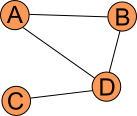
\includegraphics{graf.png}
\end{figure}

Här representeras de fyra hörnen av fyra olika cirklar, och kanterna som streck mellan de två hörn som utgör kanten.

Om en kant $(u, v) \in E$ kallar vi noderna $u$ och $v$ för \emph{grannar}. En mängd hörn $V' \subseteq V$ kallas för \emph{oberoende} om inget par av hörn i $V'$ är grannar. I figur~\ref{fig:independent_set} har hörnen i en oberoende mängd
markerats med rött.

\begin{center}
    \centering
    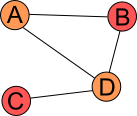
\includegraphics{oberoende_graf.png}
    \captionof{figure}{De rödfärgade noderna i grafen bildar en oberoende mängd.}
\label{fig:independent_set}
\end{center}

En partition av $V$ i $k$ oberoende mängder kallas för en $k$-\emph{färgning}. Vi kan också formulera det som att varje hörn är färgad
med en utav $k$ färger (t.ex. färgerna $\{1, 2, ..., k\}$) så att inga två grannar har samma färg.

\begin{figure}[h!]
\centering
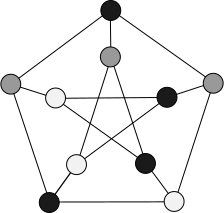
\includegraphics{giltig_petersen}
\caption{En giltig färgning av Petersens graf }
\label{fig:petersen_coloring}
\end{figure}

I figur~\ref{fig:petersen_coloring} ser vi en giltig färgning av Peterens graf med tre färger. Observera att inga två hörn som är grannar har samma färg.

\begin{figure}[h!]
\centering
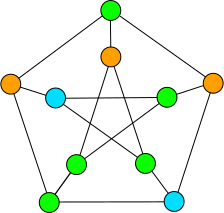
\includegraphics{ogiltig_petersen}
\caption{En ogiltig färgning}
\label{fig:invalid_coloring}
\end{figure}

Figur~\ref{fig:invalid_coloring} visar en ogiltig färgning av samma graf. Här finns det par av grannar som båda är gröna, vilket gör färgningen ogiltig.

En graf kallas för $k$-\emph{färgbar} om det existerar en $k$-färgning av grafen.

\subsection{Inklusion/exklusion}

Principen om inklusion/exklusion har många formuleringar. Den vi kommer att använda oss av är följande:

\begin{theorem}
    Givet mängderna $S_1, ..., S_n$ är antalet element i universumet $U$ som inte är ett element i någon av $S_i$ lika med
    $$\sum_{I \subseteq \{1, 2, ..., n\}}{(-1)^{|I|} \cdot |\bigcap_{i\in I}{S_i}|}$$
    Vi sätter här $\bigcap_{i \in \emptyset}{S_i} = U$.
\end{theorem}
\begin{proof}
    Om något element $x \in U$ inte är i någon av mängderna $S_i$ kommer den räknas exakt en gång, nämligen då $I = \emptyset$.

    Antag att $x \in S_i$ exakt för de $i \in I \not= \emptyset$. $x$ kommer då räknas med 

    $$\sum_{X \subseteq I}{(-1)^{|X|}} = \sum_{i=0}^{|I|}{{|I| \choose i}\cdot(-1)^i} = (1-1)^{|I|} = 0$$

    enligt binomialsatsen.
\end{proof}


\subsection{Tidskomplexitet}

När vi analyserar prestandan av våra algoritmer vill vi kunna uttrycka hur mycket tid och minne de kräver som en funktion av grafens storlek. Lite löst uttryckt
låter vi $T(G)$ vara antalet operationer som vår algoritm utför för en graf $G$, där en operation är någon ``liten'' instruktion som en dator kan utföra (t.ex.
addera två tal, läsa ett heltal ur minnet). Vi gör också det förenklade antagandet att alla sådana operationer tar uniform tid (vilket oftast inte är sant när en algoritm
körs på en riktig dator). En mer omfattande behandling av algoritmanalys finns i Knuth~\cite{Knuth1:1997}).

För två reellvärda funktioner $f$ och $g$ använder vi notationen $g(n) = O(f(n))$ om det existerar ett $C > 0, x_o$ så att för alla $x \ge x_o$ är $\frac{g(n)}{f(n)} < C$. Detta betyder rent intuitivt att $g(n)$
inte växer snabbare än $f(n)$. Vi kommer oftast använda denna asypmtotiska notation för att beskriva körtiden och minnesanvändningen för våra algoritmer.

\subsection{Kromatiska talet}

Givet en enkel graf $G = (V, E)$ vill vi bestämma det minsta antalet färger som krävs för färga grafen, dvs det minsta $k$ sådan att $G$ är $k$-färgbar.

Det minsta antalet färger som behövs för att färga en graf $G$ kallar vi det \emph{kromatiska talet} och betecknar det med $\chi(G)$. Det kromatiska talet för Petersens graf som vi såg ett exempel på är 3, vilket vi uppnår med färgningen i figur~\ref{fig:petersen_coloring}

Att bestämma det kromatiska talet är svårt att göra rent matematiskt, men för vissa klasser av grafer känner vi till det kromatiska talet, eller har olika
gränser på det kromatiska talet. T.ex. har en graf med exakt ett hörn det kromatiska talet 1, alla övriga (sammanhängande) bipartita grafer det kromatiska talet 2 och alla planära
grafer har $\chi(G)\le 4$ (det så kallade fyrfärgsteoremet).

En tämligen enkel gräns är $\chi(G) \le d + 1$, där $d$ är det största antal grannar som något hörn i grafen har.


\begin{theorem}
    I en graf där $d$ är det största antalet grannar ett hörn har är $\chi(G) \le d + 1$.
\end{theorem}

\begin{proof}
    Betrakta en tilldelning av $d+1$ färger till grafen som minimerar antalet par av grannar med samma färg. Låt $(u, v)$ vara ett sådant par.

    Eftersom $u$ har högst $d$ grannar finns det enligt lådprincipen minst en färg sådan att ingen av $u$:s grannar har den färgen. Om vi tilldelar
    $u$ den färgen minskar antalet par av grannar med samma färg. Eftersom vi hade färgat grafen så att antalet par var minimerat måste
    antagandet att ett par $(u, v)$ varit falskt, alltså är grafen korrekt färgad.
\end{proof}

Eftersom ett hörn som mest kan ha alla övriga hörn som grannar följer även

\begin{corollary}
    Om $G = (V, E)$ är en graf så gäller $\chi(G)\le|V|$.
\end{corollary}
\begin{proof}
    Det största antalet grannar ett hörn kan ha är $|V| - 1$.
\end{proof}

\subsection{Bruteforce}
Den första (och enklaste) algoritmen för att beräkna det kromatiska talet går ut på att prova alla möjliga färgningar. Notera att det finns $|V|^k$ möjliga färgningar av en graf med högst $k$ färger. Vi kan rekursivt generera alla dessa färgningar och sedan kontrollera om färgningen är giltig eller inte. Det kromatiska talet är då minimum av antalet färger hos de giltiga färgningarna. Att kontrollera om en färgning är giltig kan vi göra i $O(|E|)$ tid genom att för varje par av grannar se om de har samma färg. Detta ger oss en algoritm som går i tid $O(|E||V|^k)$ för att avgöra $k$-färgbarhet och $O(|E||V|^{d})$ för att bestämma det kromatiska talet.

Vi behöver bara testa alla $k$ upp till $d$, ty om $k > d$ är $k = d + 1$. 

En alternativ algoritm för att beräkna $\chi(G)$ är att binärsöka över $k$ och testa om grafen är $k$-färgbar. I det värsta fallet, då $\chi(G) \ge d$ kommer detta vara långsammare.
Annars kommer algoritmen att testa högst $lg (d)$ värden på $k$, alla högst $d-1$. Men $|V|^{d} \ge |V|^{d-1}\cdot{\lg(d)}$, dvs för alla möjliga värden på
det kromatiska talet förutom då $k \ge d$ kommer algoritmen vara asymptotiskt snabbare. För slumpmässiga grafer kan detta ge en kraftig förbättring. Pseudokod
för den senare algoritmen blir som följer:

\clearpage

\begin{algorithmic}[1]
    \Procedure{Color}{$G$, $A$, $i$, $k$}\Comment{Givet att de första $i-1$ hörnen har färgerna $A_k$, generera alla färgningar med högst $k$ färger.}
        \If{$i = |V| + 1$}
            \ForAll{$(u, v) \in E$}
                \If{$A_u = A_v$}
                    \State Svara $NEJ$
                \EndIf
            \EndFor
            \State Svara $JA$
        \EndIf
        \ForAll{$c$ mellan 1 och $k$}
            \State Sätt $A_i = c$
            \If{$Color(G, A, i+1, k)$}
                \State Svara $JA$
            \EndIf
        \EndFor
        \State Svara $NEJ$
    \EndProcedure

    \Procedure {ChromaticNumber}{$G$}
        \State $d \gets $högsta antalet grannar hos ett hörn.
        \State $lo \gets 0, hi \gets d+1$
        \While{$hi - lo > 0$}
            \State $mid \gets \frac{hi + lo}{2}$
            \If{$Color(G, A, 1, mid)$}
                \State $hi \gets mid$
            \Else
                \State $lo \gets mid$
            \EndIf
        \EndWhile
        \State Svara $hi$
    \EndProcedure
\end{algorithmic}

Vi kan göra en liten förbättring av algoritmen. Observera att två färgningar som är lika förutom en permutation av färgerna kommer betraktas flera gånger, trots att de för oss är ekvivalenta. Om vi inte genererar färgningar som är en färgning med permuterade färger behöver vi bara titta på alla partitioner av hörnen med högst $d$ delar. Det finns totalt $\sum_{k=0}^d{S(n, k)}$ sådana, där $S(n, k)$ är $S$ är Stirlingtalen av andra ordningen.

Denna modifikation kräver i princip endast en ändring av ``för alla $c$ mellan 1 till $\min(k, \max(A_i) + 1)$'' i proceduren som genererar färgningarna (se Knuth~\cite{Knuth4a:1997}).

\subsection{Backtracking med pruning}
I den föregående algoritmen spenderar vi mycket tid på ogiltiga färgningar. Ett bättre alternativ är \emph{backtracking med pruning}. När vi bygger upp färgningarna rekursivt kan vi ofta avgöra om färgningen är ogiltig tidigare än sista hörnet (vilket är vad vi gör i den vanliga bruteforce-algoritmen). 
Genom att kontrollera detta när vi tilldelar varje hörn sin färg kommer vi få en drastisk förbättring av körtiden. Att analysera körtiden för en sådan algoritm är generellt mycket svårt, även i slumpmässiga grafer.

\subsection{Dynamisk programmering}

Från definitionen av färgning vet vi att en delmängd av hörn kan ha samma färg om och endast om delmängden är en oberoende mängd.

Detta ger oss ett alternativ till bruteforce-algoritmerna. Antag att vi har färgat en delmängd $S$ av hörnen, och ska färga $V \setminus S$. Vi provar då att välja någon oberoende mängd $S'$ som nästa färg, och färgar $(V \setminus S) \setminus S'$. Om vi väljer den oberoende mängd som ger det bästa resultatet kan vi ställa upp en rekurrens för $\chi(G)$:

$$\chi(G[S]) = 1 + \min_{I \in I(G[S])}\{\chi(G[S \setminus I])\}$$

med

basfallet att $\chi(G) = 0$ om $G$ är den tomma grafen.

Här betyder $G[S]$ den graf som fås genom att ta mängden hörn $S$ och alla kanter som har båda ändpunkter i $S$ (kallad för den \emph{inducerade subgrafen} av $S$.

Det finns högst $2^n$ delmängder (och därmed oberoende delmängder) av en graf med $n$ hörn. Om vi bygger upp en tabell över alla delresultat
i rekurrensen får vi tidskomplexiteten

$$O(\sum_{S \subseteq V}{|I(G[S])|}) = O(\sum^n_{k=0}{{n \choose k}2^k}) = O(3^n)$$

Här har vi låtit $I(G)$ vara mängden oberoende mängder av grafen $G$.

Observera att det faktiskt inte är nödvändigt att prova att låta \emph{alla} oberoende mängder utgöra nästa färg. Det räcker med att prova alla maximala oberoende mängder. Det finns dock högst $3^{n/3}$ sådana (Miller~\cite{Miller:1960}), och de kan även listas i tid $O(3^{n/3})$ (Eppstein~\cite{Eppstein:2003}).

Med denna ändring tar algoritmen istället tid (vi har låtit $MI(G)$ vara mängden maximala oberoende mängder av grafen $G$)

$$O(\sum_{S \subseteq V}{|MI(G[S])|}) = O(\sum^n_{k=0}{{n \choose k}3^{k/3}}) = O((1 + 3^{1/3})^n) =  O(2.443^n)$$

En klar förbättring jämfört med att testa alla möjliga oberoende mängder.

\subsection{Inklusion/exklusion}

Det hittils bästa resultatet kommer av Björklund, Husfeldt och Koivisto~\cite{Bjorklund:2009}. De formulerade en formel till antalet lösningar på olika partitioneringsproblem av mängder baserat på inklusion/exklusion. Graffärgning kan som vi såg i föregående algoritm formuleras på det viset - vi vill partitionera mängden hörn i en graf i ett antal oberoende mängder.

\chapter{Metod}
\todo{Hur gjordes jämförelserna av algoritmerna; dator, operativsystem, kompilator}
\todo{Hur konstruerades testgraferna}

\chapter{Resultat}
\todo{Körtider för algoritmerna när implementationen är klar}
\chapter{Diskussion}
\todo{Analysera körtidsresultaten för algoritmerna}

\nocite{VanLint:2006}
\bibliographystyle{plain}
\bibliography{referenser}{}

\section*{Bilaga A: Implementationer av algoritmerna i C++}
\todo{Implementera algoritmerna i C++}
\section*{Bilaga B: Testgrafer}
\section*{Bilaga C: Populärvetenskaplig uppsats om graffärgning}



\end{document}
